\documentclass{article}
\usepackage[utf8]{inputenc}
\usepackage[T1]{fontenc}
\usepackage[spanish]{babel}
\usepackage{setspace}
\usepackage{geometry}
\geometry{margin=2.5cm}
\setstretch{1.2}
\usepackage{graphicx}
\usepackage[utf8]{inputenc}
\usepackage[spanish]{babel}
\usepackage{amsmath}
\usepackage{float}
\usepackage[utf8]{inputenc}
\usepackage[spanish,mexico]{babel}
\usepackage[margin=2.5cm]{geometry}
\usepackage{graphicx}
\usepackage[export]{adjustbox}
\usepackage{caption}
\usepackage{subcaption}
\usepackage{fancyhdr}
\usepackage{enumitem}
\usepackage{amsmath}
\usepackage{amssymb}
\usepackage{amsfonts}
%\usepackage{hyperref}
\usepackage[colorlinks=true, allcolors=blue]{hyperref}
\pagestyle{fancy}
\fancyhf{}

\usepackage[T1]{fontenc}   
    \usepackage{array}
    \newcommand{\tarjeta}[3]{%
      \begin{center}
      \begin{tabular}{|>{\raggedright\arraybackslash}p{7.8cm}|>{\raggedright\arraybackslash}p{4.2cm}|}
        \hline
        \multicolumn{2}{|c|}{#1} \\ \hline
        #2 & #3 \\ \hline
      \end{tabular}
      \end{center}
    }
\title{Template Facultad de Ciencias, UNAM}
\author{Yoltic Giovanni Santillan Ruiz}


\begin{document}

\thispagestyle{empty}
	
	\begin{figure}[ht]
	   \minipage{0.76\textwidth}
			
\includegraphics[width=4cm]{Logo_UNAM.png}
			\label{EscudoUNAM}
	   \endminipage
	   \minipage{0.32\textwidth}
			
\includegraphics[height=4.3cm ,width=4.3cm]{Logo_FC.png}
			\label{EscudoFC}
		\endminipage
	\end{figure}
	
	\begin{center}
	\vspace{0.8cm}
	\LARGE
	UNIVERSIDAD NACIONAL AUTÓNOMA DE MÉXICO 
	
	\vspace{0.8cm}
	\LARGE
	FACULTAD DE CIENCIAS
	
	\vspace{1.7cm}	
	\Large
	\textbf{Proyecto1MyPChat}

	\vspace{1.3cm}
	\normalsize	
	PRESENTA \\
	\vspace{.3cm}
	\large
	\textbf{Yoltic Giovanni Santillan Ruiz \\ 323124539}
	
	\end{center}
	
	\newpage



\section{Resumen}
\label{sec:resumen}

Este proyecto consta de dos sistemas independientes, el SERVIDOR y el CLIENTE, el primero tiene la finalidad de servir como medio de comunicacion entre distintos clientes usando JSON como lenguaje, mediante mensajes generales, privados, salas, cambio de estatus, listas de usuarios, etc. Mientras que el CLIENTE se encarga de la interaccion con el usuario con el fin de que pueda usar el servidor.
Para el SERVIDOR use el lenguaje de programacion C, mientras para el CLIENTE C\#\ , como resultado tenemos un sistema de comunicacion un poco primitivo pero funcional entre distintos usuarios usando el CLIENTE mediante el SERVIDOR.
\section{Introducción}
\label{sec:introduccion}

\subsection{Problema a resolver}
Los sistemas de mensajeria requieren que varios usuarios conectados mediante equipos y programas distintos puedan entrablar una comunicacion en red, esto exige un servidor que centralice y se encargue de las conexiones y el envio de mensajes, asi como clientes que se puedan comunicar con el servidor y puedan ser usados por los usuarios. El problema y el reto es que los dos programas se entiendas y que la comunicacion funcione, sin importar quien desarrollo cada componente.

\subsection{Alcance}
El alcance del proyecto no se limita a la pareja cliente-servidor
desarrollada. Gracias a que se siguió estrictamente la especificación del
protocolo que usaba JSON como lenguaje de traduccion, el cliente puede conectarse y comunicarse con los servidores
implementados por otros compañeros, y de igual forma el servidor puede atender
a los clientes de otras implementaciones. La interoperabilidad es una de las propiedades centrales del sistema y un criterio muy claro y especifico.

\subsection{Limitaciones y posibles problemas}
La principal limitación del proyecto es la experiencia de usuario del cliente.
Por falta de tiempo no se desarrolló una interfaz gráfica, por lo que toda la
interacción entre el usuario y el cliente se realiza mediante el teclado en la
terminal. Esto puede resultar confuso y poco agradable, sobre todo para
usuarios sin experiencia con este tipo de interfaces. Además, al depender de
implementaciones ajenas para la interoperabilidad, si alguien cometio un errro o hizo algo fuera del protocolo esto puede provocar fallos de comunicación un pooco dificiles de encontrar, y las diferencias de red entre equipos pueden impedir las conexiones, sobre todo si no todos son LINUX.

\subsection{Mejoras}
Una mejora que se me viene a la mente es el poder enviar imagenes, sin embargo creo que esto elevaria demasioado el nivel de dificultad.
\section{Análisis y diseño}
\label{sec:analisis-y-diseno}

Al iniciar el proyecto no se tenía experiencia previa con programación de sockets,
ni con los lenguajes C y C\#, por lo que el primer diseño fue construido un poco a
ciegas, el cual dividía el problema en los siguientes subproblemas.

\subsection{Servidor}

\subsubsection{Division en subproblemas}

\begin{itemize}
    \item \textbf{¿Cómo aceptar y atender conexiones de múltiples clientes?}

    \item \textbf{¿Dónde y cómo guardar a los usuarios conectados?}

    \item \textbf{¿Cómo evitar que dos hilos corrompan la tabla de usuarios al mismo tiempo?}

    \item \textbf{¿Cómo representar las salas de chat?}

    \item \textbf{¿Cómo interpretar los mensajes JSON que llegan del cliente?}

    \item \textbf{¿Cómo construir las respuestas del servidor?}

    \item \textbf{¿Cómo saber dónde termina un mensaje dentro del flujo de bytes de TCP?}
\end{itemize}

\subsubsection{Respuestas a los subproblemas}

\begin{itemize}
    \item Necesitaba un módulo para aceptar conexiones entrantes y mantener
    comunicación entre usuarios, esto lo hice aprendiendo de sockets e hilos~\cite{beej}, creando un hilo por cada usuario y manteniendo el servidor escuchando
    nuevas conexiones.

    \item Cada usuario debía quedar asociado a su nombre y a su socket, para poder
    enviarle mensajes en cualquier momento y para poder buscarlo por nombre
    cuando otro usuario quisiera comunicarse con él. Esto llevó a un diccionario
    de usuarios, el cual tenía de llave el nombre de usuario, 
    implementado con \texttt{uthash}~\cite{uthash}, pues C no tiene diccionarios nativos así que elegí esa que es de las más conocidas.

    \item Para hacer esto, seguí el consejo de Canek de usar mutex, así que eso
    implementé; al ser una estructura compartida entre todos los hilos de
    cliente, se protegió con un \texttt{pthread\_mutex\_t}~\cite{pthreads}, de forma que solo
    un hilo a la vez pudiera leerla o modificarla.

    \item El protocolo contempla mensajes para crear una sala, invitar usuarios,
    unirse a ella, listar sus miembros y salir de la misma, por lo que se
    necesitó una estructura análoga a la tabla de usuarios, pero para salas.
    Cada sala mantiene su propio diccionario de miembros, implementado también
    con \texttt{uthash}, cuyas entradas no almacenan una copia de los datos
    del usuario, sino su nombre y un apuntador al nodo correspondiente dentro
    de la tabla global de usuarios. De esta forma se evita duplicar la
    información y, sobre todo, se evita el problema de mantener sincronizados
    dos diccionarios independientes con los mismos datos. Para las
    invitaciones pendientes se usó una estructura equivalente, que igualmente
    guarda el nombre de usuario invitado. Al tratarse, de nuevo, de estructuras
    compartidas entre hilos, se protegieron con el mismo cuidado de acceso
    concurrente que la tabla de usuarios.

    En un inicio los diccionarios de miembros de las salas tenían sus
    apuntadores a sus propias estructuras Usuario, pero cuando me di cuenta de
    que tenía que mantenerlo sincronizado y actualizado con el diccionario
    general, y además Canek regañó a un compañero por hacer esto, decidí
    modificarlo.

    \item El protocolo especifica el formato de cada mensaje en JSON, así que se
    necesitaba un mecanismo para leer esa estructura y obtener sus campos.
    Se usó la librería \texttt{cJSON} para parsear el texto recibido y
    extraer, por ejemplo, el tipo de mensaje y sus argumentos, pues Canek especifico que no debiamos de hacer los JSON a mano.

    \item De la misma forma en que se interpreta el JSON recibido, el servidor
    necesita construir sus propias respuestas en JSON. Se usó \texttt{cJSON}
    también para este propósito, generando la cadena de texto a enviar, esto
    con un solo método que tuviera todas las posibles claves; cuando lo
    llamábamos, si no ocupábamos algunas las pasábamos como NULL, pues la idea
    original era hacer un método diferente por cada JSON que tenía que enviar,
    pero se fueron convirtiendo en DEMASIADOS, así que decidí hacer solo uno.

    \item Como TCP no garantiza que un mensaje llegue completo en una sola lectura,
    se necesitaba un criterio para separar mensajes. Se adoptó el salto de
    línea (\texttt{\textbackslash n}) como delimitador, acumulando los bytes
    recibidos en un búfer y extrayendo un mensaje completo cada vez que
    aparece el delimitador.
\end{itemize}

La Figura~\ref{fig:secuencia-identify} muestra el flujo completo de un mensaje
\texttt{IDENTIFY}, desde que llega al servidor hasta que se envía la
respuesta. El servidor recibe los bytes crudos del socket y los acumula en un
búfer hasta encontrar el delimitador \texttt{\textbackslash n}, momento en el
que extrae un mensaje completo. Ese mensaje se le pasa a
\texttt{TraduccionJson}, que usa la librería \texttt{cJSON} para parsear el
texto y obtener tanto el tipo de mensaje como sus campos —en este caso, el
\texttt{username} enviado por el cliente—, y regresa esos datos ya listos al
servidor. Con el tipo de mensaje identificado como \texttt{IDENTIFY}, el
servidor llama a \texttt{Identificar}, que bloquea el mutex de la tabla de
usuarios antes de consultarla, garantizando que ningún otro hilo pueda
modificarla al mismo tiempo. Si el nombre de usuario no existe, se agrega a la
tabla y se construye la respuesta de éxito; si ya está en uso, se construye
directamente la respuesta de rechazo. En ambos casos la construcción de la
respuesta ocurre todavía dentro de la sección protegida, y es hasta entonces
que se libera el mutex, antes de que el servidor envíe la respuesta al
cliente, esa es la logica principal de SERVIDOR, lo unico que varia es la interpretacion del JSON.

\begin{figure}[H]
    \centering
    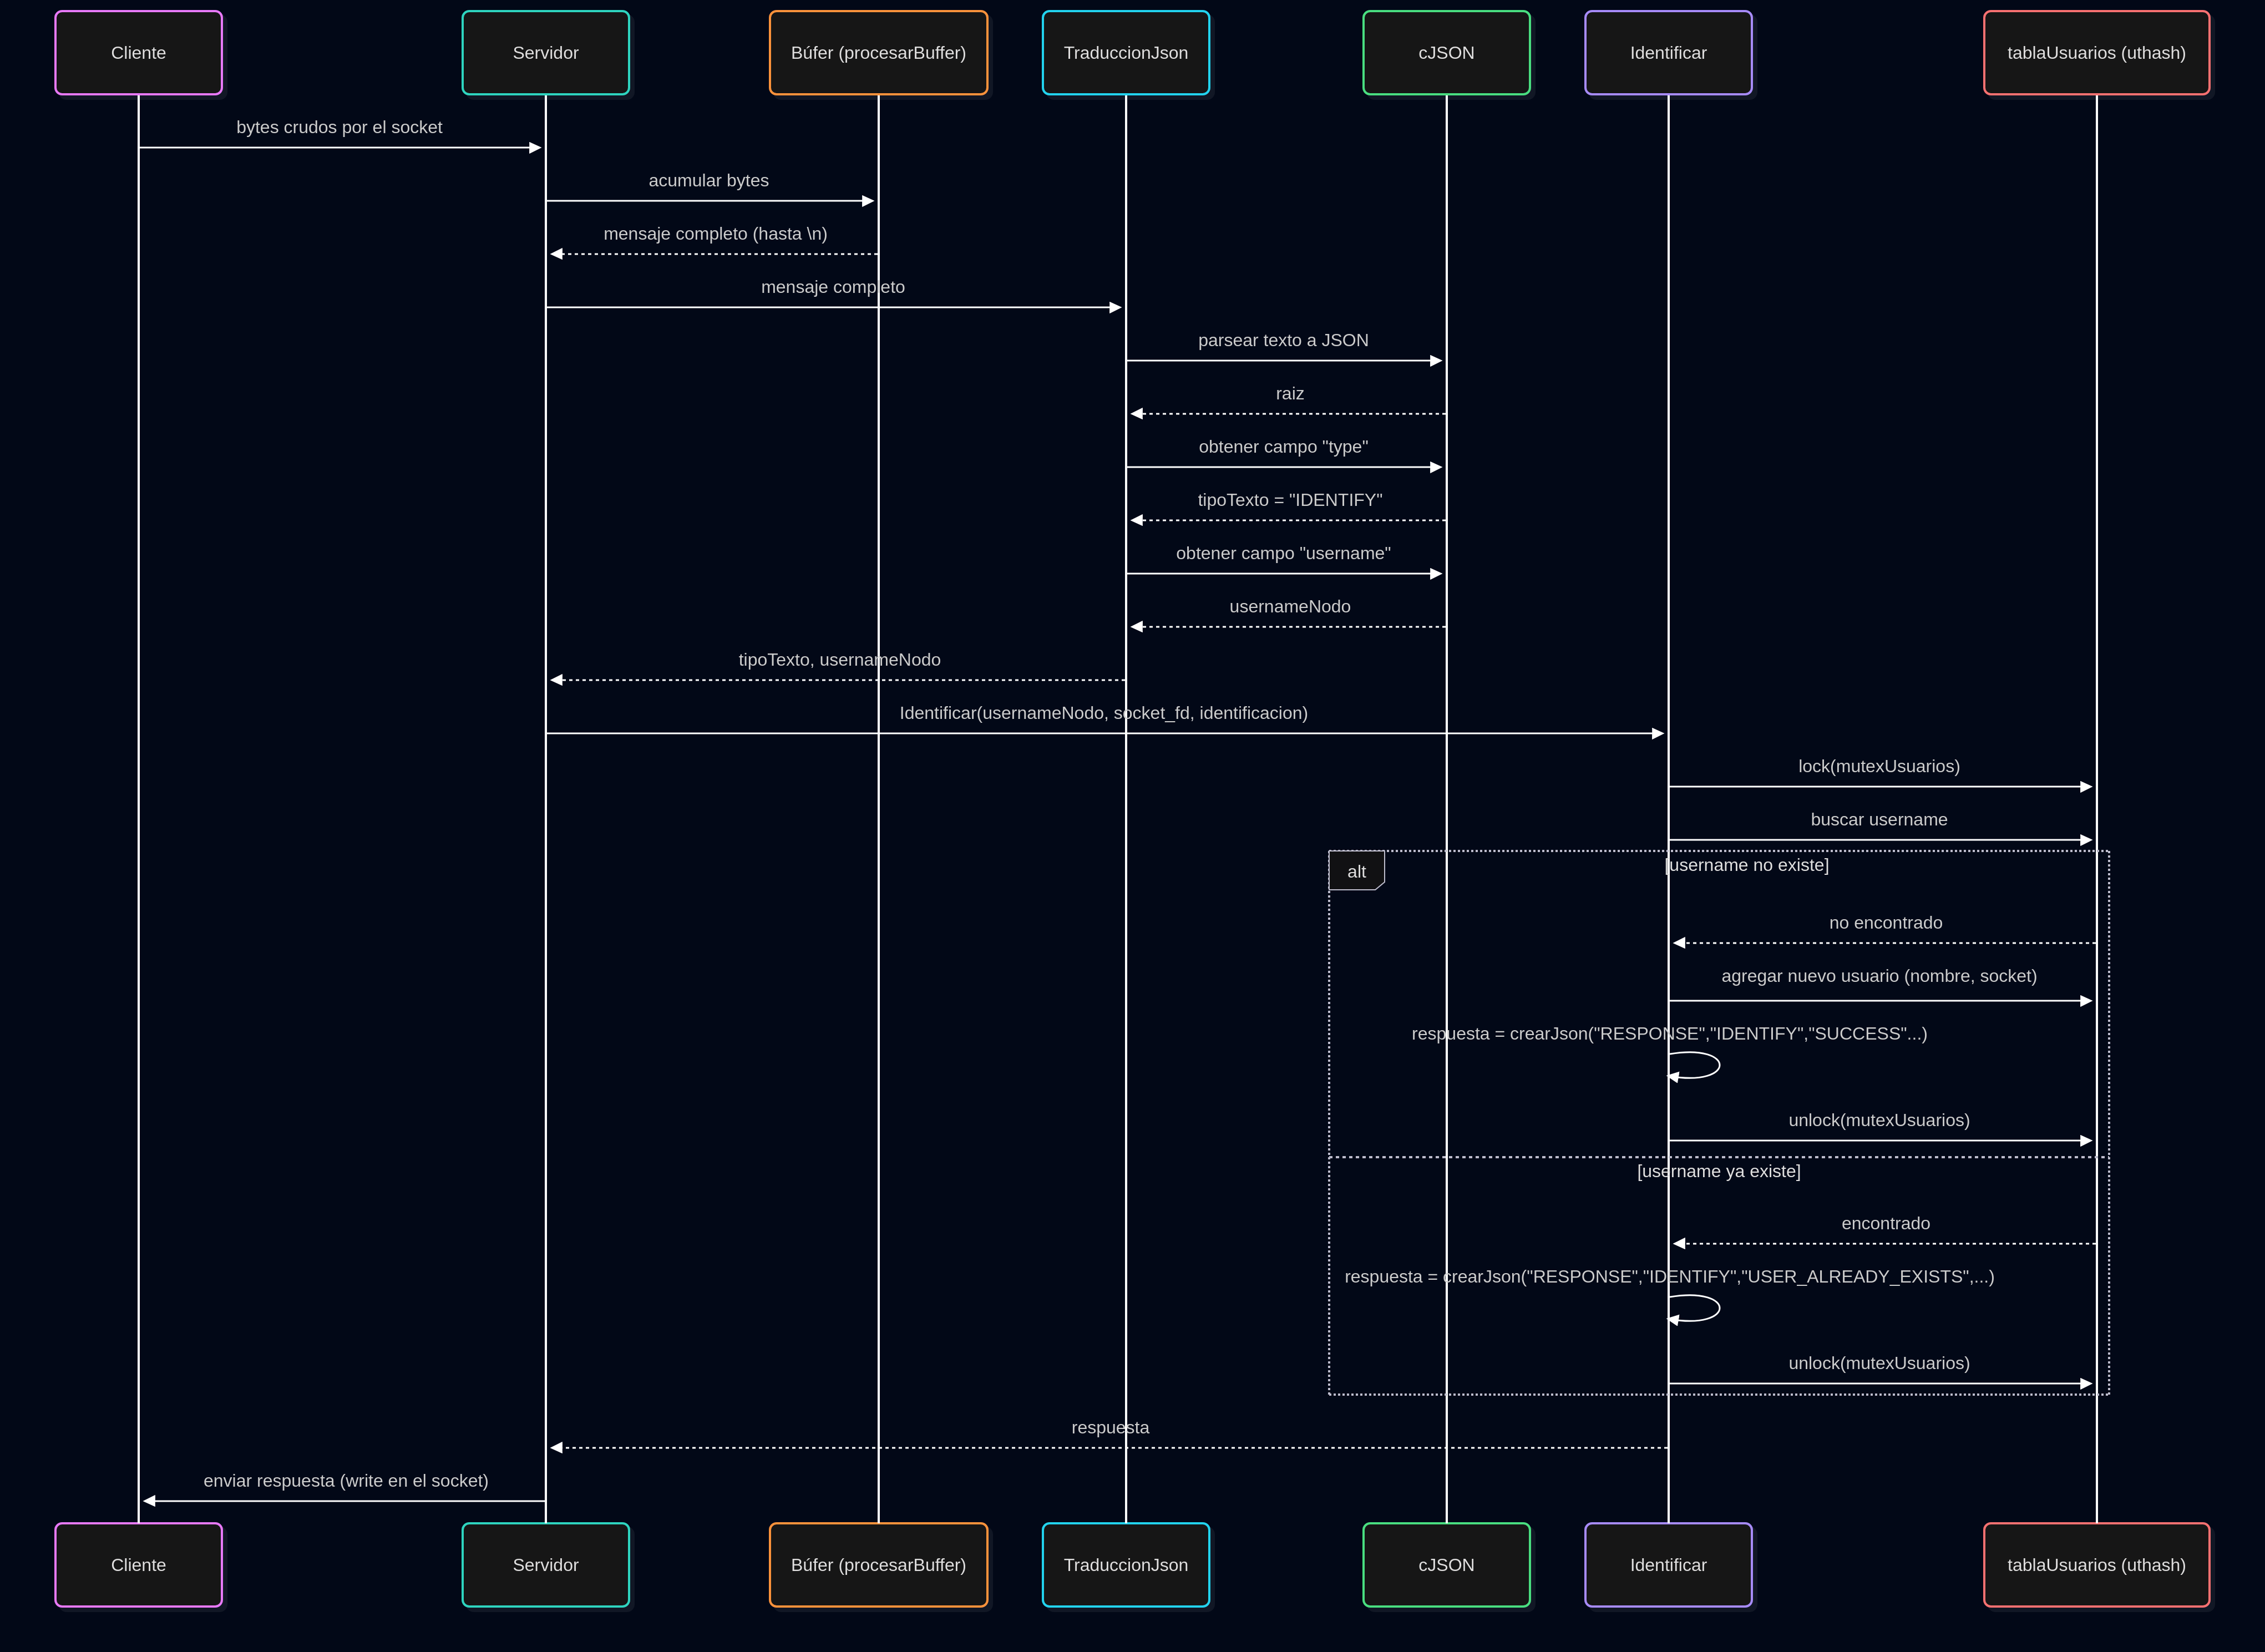
\includegraphics[width=1\textwidth]{secuencia_identify..png}
    \caption{Diagrama de secuencia del flujo IDENTIFY.}
    \label{fig:secuencia-identify}
\end{figure}

\subsubsection{Cronología}
Lo primero que hice fue compilar y ejecutar un \texttt{main} en C usando Meson
build; repito, no sabía nada de C, así que este fue el paso 0. Después
aprendí conexiones, sockets y envíos a través de la red para poder abrir un
servidor de juguete, e hice que pudiera aceptar varias conexiones mediante
hilos de ejecución. Empecé a tratar con el JSON enviado, principalmente
nombres de usuario y mensajes generales y privados, para implementar la
lista (diccionario) de usuarios. Seguí con las salas, implementando una
lista (diccionario) de salas y sus algoritmos, para pasar después a la
construcción del JSON con el que se envían las respuestas a los clientes.

\subsubsection{Notas}

\begin{itemize}
    \item No usé ningún patrón de diseño evidente; creo que para el servidor
    hubiera funcionado MVC, sin embargo, como en la vista no hay nada, porque
    el usuario no interactúa con este ejecutable, no lo vi tan necesario.

    \item No usé el patrón Iterator directamente, pues \texttt{uthash} tiene
    \texttt{HASH\_ITER}, con el cual siempre recorrí mis diccionarios, y este
    no tiene un objeto aparte que recorra el diccionario, así que técnicamente
    no sigue el patrón.

    \item Conforme fui avanzando con el protocolo y las indicaciones en base a cada mensaje del JSON, fui haciendo pruebas unitarias, aunque todas  eran de la funcion \texttt{procesarBuffer}, la cual recibia el mensaje que el cliente le enviaba, la mandaba a traducir donde se hacia la logica correspondiente y regresa la logica correspondiente, no probe conexines pero si probaba toda la logia detras.
    
\end{itemize}


\subsubsection{Tarjetas CRC del servidor}

\tarjeta{Servidor}
{Contiene el main del ejecutable\newline
 Llama a runServidor() que inicia todo}
{SocketServidor}

\tarjeta{SocketServidor}
{Abre el servidor para recibir conexiones\newline
 Administrar conexiones desprendiendo hilos\newline
 Recibir y separar mensajes completos con el delimitador \texttt{\textbackslash n}\newline
 Conservar los mensajes parciales\newline
 Enviar mensajes mediante el socket al cliente}
{IndicacionesServidor\newline TiposDeJson \newline SocketServido}

\tarjeta{IndicacionesServidor}
{interpretar los mensajes del protocolo: \texttt{IDENTIFY}, \texttt{USERS}, \texttt{STATUS}, \texttt{TEXT}, \texttt{PUBLIC\_TEXT}, \texttt{NEW\_ROOM}, \texttt{INVITE}, \texttt{ETC}\newline
 Traducir e interpretar el JSON recibido\newline
 Hacer la LOGICA (agregar a salas, listas, eliminar, crear salas, enviar mensajes, etc) en base a la interpretacion del JSON \newline
 Regresar el JSON a enviar}
{TiposDeJson\newline Salas\newline ListaDeUsuarios\newline SocketCliente}

\tarjeta{TiposDeJson}
{Crear JSON para enviar\newline
 Agregar delimitador en los JSON}
{IndicacionesServidor\newline SocketServidor}

\tarjeta{ListaDeUsuarios}
{Crear usuarios con su estructura\newline
 Diccionario de usuarios\newline
 mutex para acceso seguro en entorno multihilo}
{IndicacionesServidor\newline SocketServidor}

\tarjeta{Salas}
{Crear Sala con su estructura(Con diccionario de Invitacion y diccionario de MiembroSala)\newline
Crear MiembroSala con su estructura\newline
 Diccionario de salas\newline
 Mutex para acceso seguro en entorno multihilo}
{IndicacionesServidor\newline SocketServidor}

\subsection{Cliente}

\subsubsection{Subproblemas}

\begin{itemize}
    \item \textbf{¿Cómo validar la IP y el puerto que da el usuario, y conectarse al servidor?}

    \item \textbf{¿Cómo enviar mensajes al servidor?}

    \item \textbf{¿Cómo recibir los mensajes que llegan del servidor y saber dónde termina cada uno?}

    \item \textbf{¿Cómo evitar que el usuario mande peticiones antes de haberse identificado?}

    \item \textbf{¿Cómo traducir lo que escribe el usuario en la terminal a un mensaje del protocolo?}

    \item \textbf{¿Cómo construir el JSON correspondiente para enviarlo?}

    \item \textbf{¿Cómo traducir el JSON recibido a algo legible para el usuario?}
\end{itemize}

\subsubsection{Respuestas a los subproblemas}

\begin{itemize}
    \item Se necesitaba pedir la IP y el puerto al usuario, verificar que no
    vinieran vacíos y que el puerto fuera un número válido antes de intentar
    la conexión. Esto se hizo en \texttt{ControladorCliente}, que pide los
    datos a la vista, los valida y, si son correctos, le pide al modelo
    (\texttt{SocketCliente}) que se conecte usando \texttt{TcpClient}~\cite{tcpclient}.

    \item Se necesitaba un componente responsable únicamente de la
    comunicación por socket, sin mezclar esa responsabilidad con la
    interacción con el usuario. Esto llevó a separar \texttt{SocketCliente}
    como modelo: convierte el mensaje a bytes con UTF-8 y lo escribe en el
    \texttt{NetworkStream}, sin imprimir ni leer nada de la consola.

    \item Al igual que en el servidor, TCP no garantiza que un mensaje llegue
    completo en una sola lectura, así que se adoptó el mismo delimitador
    (\texttt{\textbackslash n}) del protocolo. \texttt{SocketCliente} acumula
    los bytes recibidos en un \texttt{string} y, cada vez que aparece el
    delimitador, extrae un mensaje completo y avisa mediante el evento
    \texttt{MensajeRecibido}, al que está suscrito el controlador.

    \item Como el protocolo exige que el usuario esté identificado antes de
    poder usar cualquier otro comando, se necesitaba bloquear el hilo de
    escritura hasta recibir la confirmación del servidor. Esto se resolvió
    con un \texttt{AutoResetEvent}: el hilo de escritura espera
    (\texttt{WaitOne}) después de enviar la identificación, y el hilo de
    escucha lo despierta (\texttt{Set}) cuando llega la respuesta del
    servidor. Esto lo hice pues yo diseñe que  el Cliente lo primero que pide hacer es enviar un nombre de usuario para con ese conectarse al servidor, pero si hay un error, el cliente vuelve a pedir un nuevo nombre de usuario, pero para saber si fue valido o no, tiene que esperar la respuesta que viene en el hilo de escritura.

    \item Lo que el usuario escribe en la terminal no es JSON, así que se
    necesitaba interpretar esa entrada y decidir qué acción del protocolo
    representa, delegando esta traducción a \texttt{IndicacionesCliente}, en un inicio lo habia hecho con comando comunes como 'escribir mensaje', 'crear nueva sala', pero estos eran dificiles de recordar asi que los hice mas sencillos, ademas de agregar una opcion 'help'

    \item Una vez interpretada la intención del usuario, se necesitaba
    construir el mensaje JSON exacto que espera el servidor según el
    protocolo, responsabilidad que también recae en \texttt{IndicacionesCliente}, donde en un inicio tambien creaba un metodo por cada JSON, sin embargo obte por la misma manera que en el SERVIDOR.

    \item Los mensajes que llegan del servidor están en JSON, por lo que se
    necesitaba interpretarlos y mostrar al usuario su contenido de forma
    comprensible en la terminal. Esto se hizo con \texttt{LecturaJson}, que
    el controlador usa tanto para mostrar la traducción del mensaje como para
    detectar casos especiales (identificación exitosa, mensaje no entendido), ademas de enviarselo a la Vista, para que el usuario los vea.
\end{itemize}

\subsubsection{Cronología}
Lo primero que hice fue lograr la conexión al servidor, para después hacer que
el cliente, mediante la terminal, pudiera mandarle cosas. Seguí con la
refactorización a MVC y, por último, con la traducción del JSON, para que el
usuario no tuviera que leer JSON.

\subsubsection{Notas}

\begin{itemize}
    \item Aquí sí usé MVC, aunque no desde el inicio; sin embargo, conforme
    fue creciendo el proyecto, supe que era necesario dividirlo, porque a
    comparación del servidor, aquí la interacción con el usuario es
    constante, y una vez que lo haces es más fácil todo lo demás, aunque la
    refactorización sí me costó bastante.

    \item Aquí hice pruebas, pero muy pocas y muy básicas: solo probé la
    separación de mensajes con \texttt{\textbackslash n} y que se guardaran
    en el búfer si no traían el delimitador, para usarlos después.

    \item Aunque el protocolo no lo dice, ni Canek lo mencionó específicamente,
    al final hice que el usuario del cliente no tuviera que leer JSON.
    Supongo que ese era el espíritu de la indicación, pues Canek solo dijo
    que el usuario no tenía que \emph{escribir} JSON, pero nunca dijo nada
    sobre leerlo.
\end{itemize}
\subsubsection{Tarjetas CRC del cliente}

\tarjeta{Cliente}
{Contiene el main del ejecutable\newline
 Llama a iniciar() para comenzar todo}
{ControladorCliente}

\tarjeta{ControladorCliente (Controlador)}
{Pedir IP y puerto\newline
 Coordinar el hilo de escucha y el de escritura\newline
 Reaccionar a cada mensaje completo del servidor, mandandolo a traducir y mandandolo a la vista para que el usuario lo vea\newline
 Sincronizar la identificación con \texttt{AutoResetEvent}\newline
 Pedir y mandar a traducir las peticiones del usuario a mensajes del protocolo}
{VistaConsola\newline SocketCliente\newline IndicacionesCliente\newline LecturaJson}

\tarjeta{SocketCliente (Modelo)}
{Guardar el estado: usuario, identificado, terminado\newline
 Conectarse al servidor por TCP\newline
 Enviar mensajes y cerrar el socket\newline
 Acumular lo recibido y separar mensajes completos con \texttt{\textbackslash n}\newline
 Avisar al controlador con el evento \texttt{MensajeRecibido}}
{ControladorCliente}

\tarjeta{VistaConsola (Vista)}
{Pedir al usuario todo lo necesario para saber a donde se quiere conectar y que quiere hacer\newline
Mostrarle al usuario que esta pasando en relacion a la comunicacion con el servidor
}
{ControladorCliente\newline IndicacionesCliente}

\tarjeta{IndicacionesCliente (Controlador)}
{Interpretar lo que el usuario escribe para saber que JSON mandar}
{ConstruccionJson\newline VistaConsola}

\tarjeta{ConstruccionJson (Modelo)}
{Construir el JSON para mardarlo al servidor}
{IndicacionesCliente}

\tarjeta{LecturaJson (Modelo)}
{Traducir lo que el servidor envio}
{ControladorCliente}

\section{Implementacion}
\label{sec:implementacion}
\subsubsection{Instrucciones de ejecución — Servidor}

\begin{verbatim}
cd SERVIDOR
meson compile -C build/
./build/Servidor
\end{verbatim}

El servidor queda escuchando en el puerto 1234.

Para correr las pruebas:
\begin{verbatim}
meson test -C build/
\end{verbatim}

\subsubsection{Instrucciones de ejecución — Cliente}
El cliente está escrito en \textbf{C\#} sobre \textbf{.NET}~\cite{dotnet}
\begin{verbatim}
cd CLIENTE/Cliente
dotnet run
\end{verbatim}

Al ejecutarse, el cliente solicita la dirección IP del servidor al que se
desea conectar, seguida del puerto y el nombre de usuario con el que se
identificará.

Para correr las pruebas:
\begin{verbatim}
cd CLIENTE/CLIENTE.Tests
dotnet test
\end{verbatim}

\subsection{Integración continua}

El repositorio incluye un flujo de \textbf{GitHub Actions} (\texttt{tests.yml})
que se ejecuta en cada \texttt{push} y \texttt{pull request}, con dos trabajos
independientes:

\begin{itemize}
    \item \textbf{Servidor}: instala Meson, Ninja, \texttt{pkgconf},
    \texttt{libcjson-dev} y \texttt{uthash-dev}; configura y compila el
    proyecto con Meson, y corre sus pruebas con \texttt{meson test}.

    Se usó la librería \texttt{cJSON}~\cite{cjson} para parsear el texto recibido...
    
    \item \textbf{Cliente}: instala el SDK de .NET 8.0 y corre las pruebas
    del proyecto \texttt{CLIENTE.Tests} con \texttt{dotnet test}.
\end{itemize}

\section{Conclusiones}
\label{sec:conclusiones}
\subsection{Servidor}
Un punto muy importante es que programar en C es bastante complicado: el uso y
la liberación de memoria complica mucho la cosa, y que no haya \texttt{string}
tampoco ayuda; que sea un lenguaje estructurado y no orientado a objetos te
nubla la vista. La próxima vez que Canek dé un punto extra por hacerlo en un
lenguaje me la voy a pensar un poco más.

El manejo del mutex fue de las cosas más complicadas que tuve; a veces se me
olvidaba desbloquearlo y el programa moría.

Me hubiera gustado hacer pruebas de conexiones, pero investigué un poco y
estaba bastante complicado, y el tiempo no me dio. Cabe aclarar que hacer
pruebas ayuda demasiado: Canek en semestres anteriores las recomendaba y nunca
las había hecho, pero me ayudaron a detectar muchísimos bugs, y saber
específicamente cuál era el problema. Además, otra cosa que
mejoraría es que mi servidor terminara bien, algo que tampoco pude lograr.

Aunque creo que no era muy necesario usar MVC, me hubiera gustado
implementarlo también; creo que es una buena práctica, aunque, repito, aquí no
tenía mucha utilidad.

\subsection{Cliente}
Hacer el cliente en C\# fue mucho más fácil, de verdad: al inicio, cuando se
trataba de conexiones, lo que en C me tomaba 3 horas en C\# me salía en 45
minutos. Sin embargo, me hubiera gustado hacer una interfaz gráfica; lo
intenté, pero ya no me metí de lleno por el tiempo. Otra cosa que me hubiera
gustado agregar eran pruebas más variadas y profundas; hubieran sido de mucha
ayuda.
\bibliographystyle{plain}    
\bibliography{referencias}
\end{document}
